\documentclass[11pt,a4paper]{article}

\usepackage[margin=2.3cm]{geometry}
\usepackage[T1]{fontenc}
\usepackage{lmodern}
\usepackage{microtype}
\usepackage{xcolor}
\usepackage{booktabs}
\usepackage{tabularx}
\usepackage{longtable}
\usepackage{array}
\usepackage{listings}
\usepackage{tikz}
\usetikzlibrary{arrows.meta,positioning,fit,backgrounds}
\usepackage{amsmath}
\usepackage{hyperref}

\definecolor{accent}{HTML}{3B5BDB}
\definecolor{codebg}{HTML}{F5F6F8}
\definecolor{good}{HTML}{2B8A3E}
\definecolor{bad}{HTML}{C92A2A}
\hypersetup{colorlinks=true,linkcolor=accent,urlcolor=accent,citecolor=accent}

\lstset{
  basicstyle=\ttfamily\small,
  backgroundcolor=\color{codebg},
  frame=single, rulecolor=\color{codebg},
  breaklines=true, breakatwhitespace=false,
  columns=fullflexible, keepspaces=true,
  showstringspaces=false, upquote=true,
  xleftmargin=4pt, xrightmargin=4pt, aboveskip=8pt, belowskip=8pt
}
\lstdefinelanguage{json}{morestring=[b]", stringstyle=\color{accent!70!black}}

% file / function names: monospace, breakable after / _ . so long names never overflow
\makeatletter
\g@addto@macro\UrlBreaks{\do\_\do\.\do\-}
\makeatother
\urlstyle{tt}
\newcommand{\file}[1]{\nolinkurl{#1}}
\newcommand{\fn}[1]{\nolinkurl{#1}}
\emergencystretch=2.5em
\newcolumntype{L}{>{\raggedright\arraybackslash}X}
\setlength{\parskip}{4pt}

\title{\textbf{AutoGrader: A Rule-Driven Evaluator for C Programs}\\[4pt]
\large Design and implementation report: what was built, where, and how}
\author{}
\date{October 2026}

\begin{document}
\maketitle

\begin{abstract}
\noindent AutoGrader is an agent that takes a student's C submission and an instructor-written
rules file, compiles and runs the program inside a sandbox with fixed time and memory limits, evaluates
every metric in the rules with its own analyzer, and returns one weighted grade together with
feedback. For an incorrect program, the feedback gives a concrete failing input with the expected
output beside it, a sanitizer diagnosis and an explanation. The backend is Django; the frontend is plain
HTML and CSS. Readability is judged by an LLM on Groq, and a locally running Ollama \texttt{qwen3:4b}
generates adversarial test inputs, tutor-style explanations and AI-written reference solutions for
copy detection. Originality is measured on an \emph{abstract structural} representation of the code. The
central contract (\emph{same submission + same rules $\rightarrow$ same grade}) was verified
experimentally: 9 sample submissions graded 3 times each gave identical grades, metric scores and
flags.
\end{abstract}

\tableofcontents
\newpage

%=====================================================================
\section{Goal and the reproducibility contract}
%=====================================================================
Grading programs by hand is slow, inconsistent and does not scale. The assignment asks for an agent that
does the whole job unattended:

\begin{enumerate}
  \item \textbf{run} the submission safely, under fixed time and memory limits, surviving programs that
        crash or never halt;
  \item \textbf{read} the grading rules from a file kept \emph{outside} the agent's source code;
  \item \textbf{evaluate} each metric with its own analyzer and combine the results into one grade using
        the weights in the rules;
  \item \textbf{produce feedback}, including a specific failing input with the expected output, memory-leak
        reports and profiling;
  \item \textbf{flag} suspected copying from peers, online resources or LLMs;
  \item state the \textbf{usefulness} and \textbf{limitations} of the agent with 3--4 concrete examples each.
\end{enumerate}

The fixed requirement is the \textbf{contract}: the same submission judged under the same rules must
receive the same grade every time. Section~\ref{sec:repro} describes how this is achieved even though
LLMs and wall-clock timings are inherently noisy.

\subsection{Where each requirement is implemented}

\begin{longtable}{@{}>{\raggedright\arraybackslash}p{4.3cm}>{\raggedright\arraybackslash}p{5.2cm}>{\raggedright\arraybackslash}p{5.6cm}@{}}
\toprule
\textbf{Requirement} & \textbf{Implementation} & \textbf{Location} \\
\midrule
\endhead
Safe execution, time/memory limits, crash and hang survival & Process-group sandbox, rlimits, memory polling, file-based I/O & \file{engine/sandbox.py} (\fn{run}, \fn{compile_c}) \\
Rules outside the code & JSON rules files, validated at load time and in the web editor & \file{rules/*.json}, \file{engine/agent.py} (\fn{validate_rules}) \\
One analyzer per metric & Plug-in registry, 9 analyzers & \file{engine/analyzers/} \\
Weighted overall grade & Collation in rules order & \file{engine/agent.py} (\fn{Agent._grade}) \\
Failing input + expected output & Hidden tests, generated corner cases, reference-solution oracle & \file{io_tests.py}, \file{edge_case_runner.py}, \file{engine/context.py} \\
Counter-test generation (corner cases) & Category generators + LLM-proposed adversarial inputs & \file{engine/inputs.py}, \file{edge_case_runner.py} \\
Memory leaks / UB (valgrind/asan) & ASan + UBSan; macOS \texttt{leaks}; LeakSanitizer/valgrind on Linux & \file{sanitizer_run.py} \\
Profiling & Per-test CPU, wall time, peak memory; scaling curve & \file{sandbox.py}, \file{complexity_estimator.py} \\
Plagiarism / LLM-copy flag & Abstract structural fingerprints, AI-generated corpus & \file{similarity_flag.py}, \file{engine/clexer.py} \\
Readability via Groq & Rubric prompt, JSON output, cached & \file{llm_review.py}, \file{engine/llm.py} \\
Ollama \texttt{qwen3:4b} & Counter-tests, tutor explanations, AI reference solutions & \file{edge_case_runner.py}, \file{agent.py}, \file{similarity_flag.py} \\
Usefulness \& limitations & Included in every report & \file{engine/usefulness_limitations.json} \\
Django backend, HTML/CSS frontend & App with worker, views, templates, one stylesheet & \file{grader/}, \file{autograder_site/} \\
Unattended end-to-end run & CLI, management command, HTTP API & \file{engine/__main__.py}, \file{grader/management/commands/grade.py} \\
\bottomrule
\end{longtable}

%=====================================================================
\section{Architecture}
%=====================================================================
The system is split into a \textbf{framework-independent engine} (\file{engine/}) and a
\textbf{Django web application} (\file{grader/}). The engine can be used on its own from the command
line; Django only stores submissions, queues work and renders reports.

\begin{figure}[h]
\centering
\resizebox{\textwidth}{!}{%
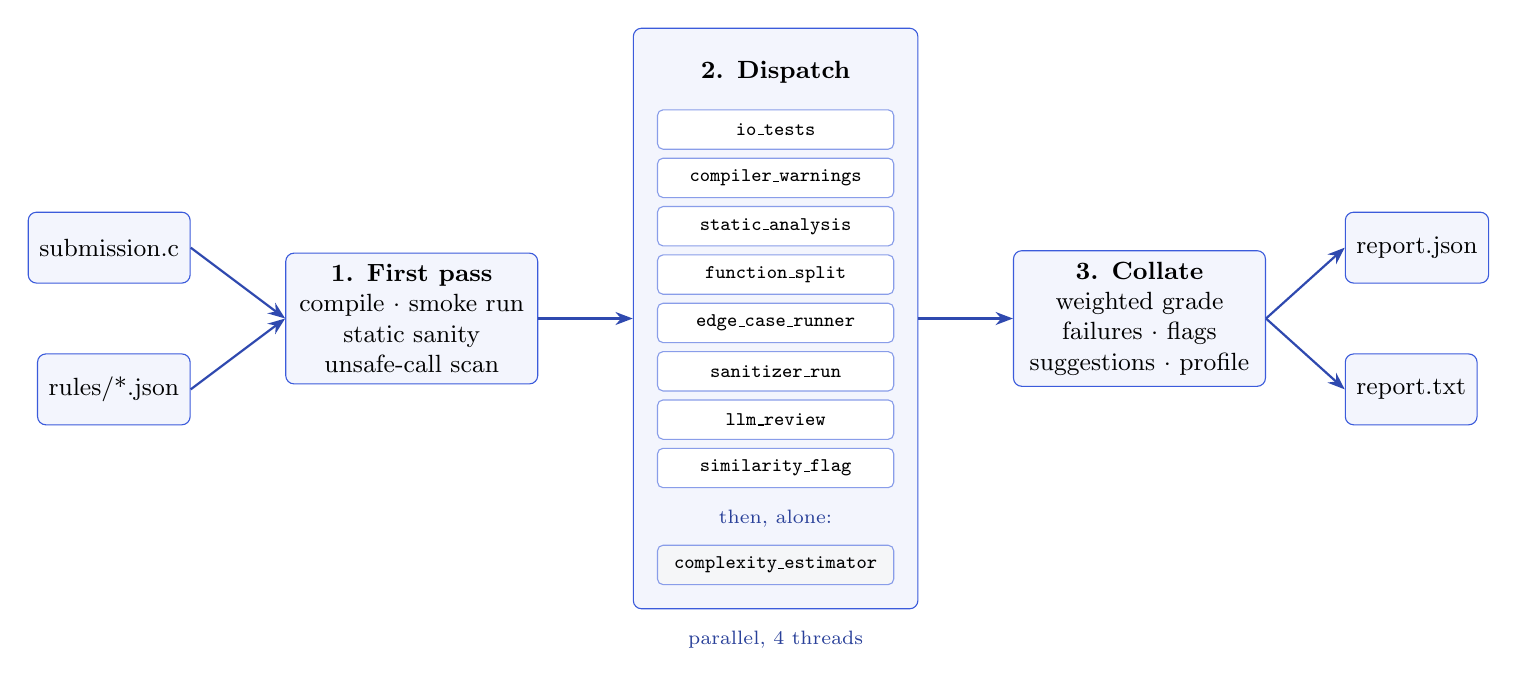
\begin{tikzpicture}[
  box/.style={draw=accent, rounded corners=3pt, fill=accent!6, align=center, font=\small, minimum height=9mm, inner sep=4pt},
  an/.style={draw=accent!60, rounded corners=2pt, fill=white, font=\scriptsize\ttfamily, minimum width=30mm, minimum height=5mm, inner sep=1.5pt},
  arr/.style={-{Stealth[length=2.2mm]}, thick, accent!80!black}]
  % analyzers column
  \node[font=\small\bfseries] (dt) at (0,0) {2. Dispatch};
  \node[an, below=2mm of dt] (a1) {io\_tests};
  \node[an, below=1mm of a1] (a2) {compiler\_warnings};
  \node[an, below=1mm of a2] (a3) {static\_analysis};
  \node[an, below=1mm of a3] (a4) {function\_split};
  \node[an, below=1mm of a4] (a5) {edge\_case\_runner};
  \node[an, below=1mm of a5] (a6) {sanitizer\_run};
  \node[an, below=1mm of a6] (a7) {llm\_review};
  \node[an, below=1mm of a7] (a8) {similarity\_flag};
  \node[font=\scriptsize, text=accent!70!black, below=1.5mm of a8] (sep) {then, alone:};
  \node[an, below=1mm of sep, fill=codebg] (a9) {complexity\_estimator};
  \begin{scope}[on background layer]
    \node[draw=accent, rounded corners=3pt, fill=accent!6, inner sep=3mm, fit=(dt)(a1)(a9)] (disp) {};
  \end{scope}
  \node[font=\scriptsize, text=accent!70!black, below=1.5mm of disp] {parallel, 4 threads};
  % first pass and inputs
  \node[box, left=12mm of disp, minimum width=32mm] (fp) {\textbf{1. First pass}\\compile $\cdot$ smoke run\\static sanity\\unsafe-call scan};
  \node[box, left=12mm of fp, yshift=9mm] (sub) {submission.c};
  \node[box, left=12mm of fp, yshift=-9mm] (rules) {rules/*.json};
  % collate and outputs
  \node[box, right=12mm of disp, minimum width=32mm] (col) {\textbf{3. Collate}\\weighted grade\\failures $\cdot$ flags\\suggestions $\cdot$ profile};
  \node[box, right=10mm of col, yshift=9mm] (json) {report.json};
  \node[box, right=10mm of col, yshift=-9mm] (txt) {report.txt};
  \draw[arr] (sub.east) -- (fp.west);
  \draw[arr] (rules.east) -- (fp.west);
  \draw[arr] (fp) -- (disp);
  \draw[arr] (disp) -- (col);
  \draw[arr] (col.east) -- (json.west);
  \draw[arr] (col.east) -- (txt.west);
\end{tikzpicture}}
\caption{Coordinator pipeline implemented in \file{engine/agent.py}.}
\end{figure}

\subsection{Project layout}
\begin{lstlisting}[basicstyle=\ttfamily\footnotesize]
autograder/
  engine/                 framework-independent agent
    agent.py              coordinator: rules validation, first pass, dispatch, collation
    sandbox.py            compile + run under time / memory / output limits
    context.py            shared state: binaries, reference oracle, tests, seeded RNG
    inputs.py             input_format -> deterministic edge-case generation + validation
    clexer.py             C lexer, abstract token stream, control skeleton, loop depth
    llm.py                Groq + Ollama clients behind a content-addressed cache
    explain.py            deterministic "WHY" explanations + sanitizer root-cause hints
    sanitizers.py         ASan / LSan / UBSan report parser (clang and gcc)
    launcher.c            Linux run launcher (exact rusage, rlimits in C)
    report.py             plain-text student report
    usefulness_limitations.json
    analyzers/            base.py + one module per analyzer (plug-ins)
    __main__.py           CLI: python -m engine
  grader/                 Django app: models, services (worker), views, templates, CSS
    management/commands/grade.py
  autograder_site/        Django settings and root URLs
  rules/                  instructor rules (add_two_integers.json, sum_array.json)
  problems/               statements + reference solutions
  tests/                  hidden tests (NN.in / NN.out)
  submissions/            sample submissions; web uploads in submissions/<problem>/uploads/
  corpus/llm_generated/   qwen3-generated solutions used for AI-copy detection
  reports/                generated JSON + text reports
  scripts/check_reproducibility.py, scripts/setup_linux.sh
  Dockerfile, docker-compose.yml   Linux image (Ubuntu 24.04, gcc 13)
  .cache/llm/             cached LLM responses (part of the grading record)
\end{lstlisting}

%=====================================================================
\section{The rules file}
%=====================================================================
Rules are plain JSON in \file{rules/}. They contain everything the agent needs, so adding a metric,
changing a weight or a threshold, or defining a new problem never requires touching the engine.
\file{rules/add_two_integers.json} reproduces the assignment's example and adds the fields the
agent needs in order to \emph{generate} its own tests:

\begin{lstlisting}[language=json]
{
  "problem": "add_two_integers",
  "statement_file": "problems/add_two_integers/statement.md",
  "reference_solution": "problems/add_two_integers/reference.c",
  "time_limit_s": 1,
  "memory_limit_mb": 64,
  "compile_flags": "-O2 -Wall -Wextra -std=c11",
  "compare": "tokens",
  "sample_input": "7 5\n", "sample_output": "12\n",
  "input_format": {"lines": [[{"name": "a", "type": "int"}, {"name": "b", "type": "int"}]]},
  "metrics": [
    {"name": "correctness", "analyzer": "io_tests", "weight": 0.20,
     "params": {"testset_dir": "tests/add/"}},
    {"name": "logical", "analyzer": "edge_case_runner", "weight": 0.10,
     "params": {"cases": ["negatives", "zero", "int_overflow", "whitespace", "llm"]}},
    {"name": "readability", "analyzer": "llm_review", "weight": 0.10,
     "params": {"model": "openai/gpt-oss-120b", "temperature": 0, "seed": 42}},
    ...
  ]
}
\end{lstlisting}

\noindent\begin{tabularx}{\textwidth}{@{}>{\raggedright\arraybackslash}p{3.9cm}L@{}}
\toprule
\textbf{Key} & \textbf{Meaning} \\
\midrule
\texttt{problem}, \texttt{statement\_file} & Name and problem text. The text is given to the LLM analyzers. \\
\texttt{reference\_solution} & Instructor's C solution, used as the \emph{oracle} that produces the expected output for generated inputs. \\
\texttt{time\_limit\_s}, \texttt{memory\_limit\_mb} & Sandbox limits for each run. \\
\texttt{input\_format} & Typed stdin layout: lines of fields with \texttt{type} (\texttt{int}, \texttt{long}, \texttt{uint}, \texttt{float}, \texttt{word}), optional \texttt{min}/\texttt{max}, and \texttt{repeat} for arrays sized by another field. \\
\texttt{compare} & Output comparison: \texttt{tokens} (default, whitespace-insensitive), \texttt{lines}, \texttt{exact}, \texttt{float:1e-6}. \\
\texttt{metrics[]} & \texttt{name}, \texttt{analyzer}, \texttt{weight}, \texttt{params}. Weights are normalised if they do not sum to 1. \\
\bottomrule
\end{tabularx}

\paragraph{Validation.} \fn{validate_rules} in \file{engine/agent.py} rejects a missing or empty metric list,
unknown analyzers (listing the available ones), duplicate metric names, negative or non-numeric weights,
non-object params and all-zero weights. The same function runs when the web editor saves a file, so an
invalid rules file can never be stored through the UI.

A second rules file, \file{rules/sum_array.json}, defines a harder problem (sum of $n \le 10^6$ integers,
required $O(n)$) so that complexity, leak and copy detection have something real to detect.

%=====================================================================
\section{Safe execution: the sandbox}
%=====================================================================
\file{engine/sandbox.py} compiles and runs untrusted code. \fn{compile_c} invokes the system compiler
(\texttt{cc}: Apple clang on macOS, gcc on most Linux distributions; it falls back to \texttt{gcc} or \texttt{clang},
and \texttt{AUTOGRADER\_CC} overrides it) and parses every
\texttt{file:line:col: warning|error: message [-Wflag]} diagnostic into structured data.

\fn{run} executes a binary with these guarantees:
\begin{itemize}
  \item \textbf{Time limit = CPU time} (user + sys), as on competitive-programming judges, so machine load cannot
        turn a correct program into a timeout. \texttt{RLIMIT\_CPU} kills spinning programs; a wall-clock
        \emph{backstop} of $3\times$ the limit $+\,1$\,s kills programs that hang without using CPU. The child runs in
        its own session, and the whole process group is killed with \texttt{SIGKILL}, so forked children die too.
  \item \textbf{Memory limit} on \emph{resident} memory. macOS ignores \texttt{RLIMIT\_AS} (we verified that
        \fn{setrlimit} fails), so the parent polls the child's physical footprint every 2--10\,ms via
        \fn{proc_pid_rusage} in \texttt{libproc} (class \fn{_MacFootprint}). On Linux it polls \texttt{VmRSS} in
        \file{/proc/<pid>/status}, with \texttt{RLIMIT\_AS} at $2\times$ limit $+\,64$\,MB as a safety net. A cap at the
        limit itself would make \texttt{malloc} fail on untouched virtual reservations and turn an MLE into a crash.
        The program's \texttt{ru\_maxrss} is checked after the run as a second line of defence.
  \item \textbf{Output limit:} \texttt{RLIMIT\_FSIZE} on the redirected output (\texttt{SIGXFSZ} $\rightarrow$ OLE).
  \item \textbf{No core dumps}, a private temporary working directory, and a scrubbed environment
        (\texttt{PATH=/usr/bin:/bin}, \texttt{LANG=C}).
  \item \textbf{Files instead of pipes} for stdin/stdout/stderr, so a program that floods its output cannot
        deadlock the grader.
\end{itemize}

Each run returns a \fn{RunResult}: stdout, stderr, exit code, signal name, flags for timeout, memory and
output limits, wall time, CPU time (user+sys from \fn{os.wait4}) and peak memory. Its \fn{verdict} property
maps these onto the judge verdicts \texttt{OK}, \texttt{TLE}, \texttt{MLE}, \texttt{OLE} and \texttt{RE}.

\paragraph{Linux launcher.} On Linux, a child forked from the grader inherits the grader's own memory peak in
\texttt{ru\_maxrss} across \texttt{exec}. In testing, a 1\,MB program was reported at 30--40\,MB, and once the
long-running grader grew past 64\,MB \emph{every} test was marked ``memory limit exceeded''. On Linux, programs
are therefore started through \file{engine/launcher.c}, a 60-line C program compiled once on first use
(\fn{_launcher}). It forks the student program from a tiny process, applies the rlimits in C (replacing Python's
\fn{preexec_fn}, which is not thread-safe while analyzers run in parallel), writes the program's pid for memory
polling, and reports the program's own \fn{wait4} status, CPU time and peak memory. With the grader holding
300\,MB, a 1\,MB program is now reported at 1.25\,MB, a 100\,MB allocation is killed as MLE and a 40\,MB one passes.

Additionally, the first pass statically refuses to execute programs that call \texttt{system},
\texttt{fork}, \texttt{exec*}, \texttt{popen}, \texttt{socket}, \texttt{kill}, \texttt{unlink}, \texttt{remove} and similar
(\texttt{DANGEROUS\_CALLS} in \file{engine/clexer.py}).

%=====================================================================
\section{The coordinator}
%=====================================================================
\fn{Agent.grade} in \file{engine/agent.py} creates a private work directory, builds a \fn{Context}
(\file{engine/context.py}) shared by all analyzers, and runs three phases.

\subsection{Phase 1: first pass (cheap sanity sweep)}
\fn{Agent._first_pass}:
\begin{enumerate}
  \item \textbf{Compile check} with the rules' \texttt{compile\_flags} (default \texttt{-O2 -Wall -Wextra -std=c11}).
  \item \textbf{Smoke run} on the sample input under the rule limits.
  \item \textbf{Static sanity:} \texttt{main} present, an input call (\texttt{scanf}, \texttt{getchar}, \texttt{fgets} \ldots),
        an output call (\texttt{printf}, \texttt{puts} \ldots), \texttt{return} inside \texttt{main}, and the unsafe-call scan.
\end{enumerate}
If the smoke run times out, the report gets a \texttt{suspected\_infinite\_loop} flag; the execution-based
analyzers (correctness, logical, complexity, memory safety) are \emph{skipped with score 0}, while the
source-only analyzers (syntax, structure, modularity, readability, originality) still run, producing a
partial report, exactly as described in the assignment. A compile failure or an unsafe call has the same effect.

\subsection{Phase 2: dispatch}
Every metric is mapped to its analyzer class through the registry. Analyzers that need a binary are
skipped if the first pass failed. The rest run in a \fn{ThreadPoolExecutor} with four workers; analyzers
marked \fn{timing_sensitive} (the complexity estimator) run \emph{alone afterwards}, so parallel work does
not distort CPU timings. An exception inside an analyzer is caught and turned into a score of 0 with
the error as evidence, so one faulty analyzer cannot destroy the report.

\subsection{Phase 3: collation and the grade}
Results are collected \emph{in rules order}, never in completion order. With normalised weights
$w_i$ and analyzer scores $s_i \in [0,1]$:
\[
  \text{grade} \;=\; 100 \cdot \frac{\sum_i w_i\, s_i}{\sum_i w_i}.
\]
Collation also merges and de-duplicates failures from all analyzers (keyed by input), adds the AI-tutor
explanations (Section~\ref{sec:llm}), ranks suggestions by the points the corresponding metric lost,
builds a profile from the per-test timings and the scaling curve, and records hashes and tool versions.

%=====================================================================
\section{The analyzers}
%=====================================================================
Analyzers subclass \fn{Analyzer} in \file{engine/analyzers/base.py}, declare \fn{needs_binary} and
\fn{timing_sensitive}, and return a \fn{Result} with a score in $[0,1]$, a feedback string, raw evidence,
failures, suggestions, flags and a one-line verdict. The \fn{@register} decorator adds them to
\fn{REGISTRY}, which is how rules refer to them by name.

\subsection{\texttt{io\_tests}: correctness (\texttt{io\_tests.py})}
Runs every \texttt{NN.in} in \texttt{testset\_dir}, compares the output with \texttt{NN.out} (or \texttt{.ans},
or the reference solution's output if no answer file exists), and records a verdict, CPU time, wall time and
peak memory per test. Every failure is explained by \fn{heuristic} in \file{engine/explain.py} and
re-run under ASan+UBSan by \fn{sanitizer_hint}, which returns the root cause, e.g.
\emph{runtime error at line 5: signed integer overflow: 2147483647 + 1 cannot be represented in type 'int'}.
\textbf{Score:} passed / total.

\subsection{\texttt{compiler\_warnings}: syntax (\texttt{compiler\_warnings.py})}
Compiles with the rule's flags, but with \texttt{-Werror} removed so warnings are counted individually instead
of collapsing into one error. It reports whether the build \emph{would} fail under \texttt{-Werror}.
\textbf{Score:} $\max(0,\,1 - 0.1 \cdot \#\text{distinct warnings})$, and 0 on compile errors.

\subsection{\texttt{static\_analysis}: structure (\texttt{static\_analysis.py})}
Uses \textbf{lizard} for per-function cyclomatic complexity and length, compared with
\texttt{max\_cyclomatic} and \texttt{max\_function\_length}, plus deterministic token-level checks: comments and a
header comment, single-block code, mutable globals, \texttt{goto}, long lines, magic numbers, and
\texttt{cppcheck} findings if \texttt{cppcheck} is installed.
\textbf{Score:} $1 - \sum \text{deductions}$ with 0.2 per over-complex or over-long function, 0.2 for no comments
(0.1 for a missing header comment), 0.1 for single-block code, 0.1 per global (max 0.2), 0.1 for \texttt{goto},
0.05 for long lines, 0.05 for $\ge 3$ magic numbers, 0.05 per cppcheck issue (max 4).

\subsection{\texttt{function\_split}: modularity (\texttt{function\_split.py})}
Counts functions (lizard), helpers other than \texttt{main}, the share of code lines in \texttt{main}, and
helpers that are never called.
\textbf{Score:} 1 if $n \ge$ \texttt{min\_functions}, else $0.3 + 0.7\min(1, h/(\texttt{min}-1))$; capped at 0.3 when
helpers are expected but absent (so \texttt{add.c} gets 3/10, as in the assignment); $-0.2$ if \texttt{main} holds more
than 75\,\% of the code; $-0.1$ for unused helpers.

\subsection{\texttt{edge\_case\_runner}: logic and counter-tests}
This analyzer \textbf{generates counter test cases}. \fn{InputFormat.category} in \file{engine/inputs.py}
builds deterministic inputs per category from the \texttt{input\_format}:

\noindent\begin{tabularx}{\textwidth}{@{}>{\raggedright\arraybackslash}p{3.3cm}L@{}}
\toprule
\texttt{zero} & all values 0; zero mixed with other values; the minimum size \\
\texttt{negatives} & $-1$, small and large negatives (only if the format allows them) \\
\texttt{int\_overflow} & patterns $[\max]$, $[\min]$, $[\max,1]$, $[\min,-1]$, $[\max,\min]$ for full-range integer fields \\
\texttt{boundaries} & every field at its declared minimum and maximum; minimum and maximum sizes \\
\texttt{random} & seeded random instances, small and full range \\
\texttt{whitespace} & the same data with tabs, multiple spaces, blank lines, missing trailing newline \\
\texttt{large}, \texttt{single}, \texttt{empty} & maximum size, $n=1$, $n=0$ \\
\texttt{llm} & \texttt{qwen3:4b} reads the statement \emph{and the student's code} and proposes inputs likely to break \emph{this} program \\
\bottomrule
\end{tabularx}

The random generator for each category is seeded from \texttt{sha256(rules\_hash + category)}
(\fn{Context.rng}), so every run produces byte-identical inputs. LLM-proposed inputs are validated by
\fn{InputFormat.validate} (token count, types, ranges) before use. This was necessary because qwen3 often
proposed a single number for a two-integer format. Expected outputs come from the compiled
\textbf{reference solution} (\fn{Context.expected}); inputs the reference rejects are not counted. Without a
reference solution the analyzer checks robustness only (no crash, hang or sanitizer report).
\textbf{Score:} passed / total, with per-category breakdown and targeted suggestions.

\subsection{\texttt{complexity\_estimator}: time efficiency (\texttt{complexity\_estimator.py})}
\textbf{Empirical part.} For each size $n$ in \texttt{sizes}, an input is generated with the size field set to $n$
(\fn{InputFormat.sized_input}). The program runs \texttt{repeats} times and the \textbf{minimum CPU time} is kept
(the minimum is the most noise-robust estimator). The smallest size is used as the baseline, and a
least-squares slope of $\log(t_n - t_0)$ against $\log n$ is fitted, ignoring points below a 4\,ms noise floor.
Slope bands map to classes: $<0.35 \rightarrow O(1)/O(\log n)$, $<1.35 \rightarrow O(n)/O(n\log n)$,
$<2.4 \rightarrow O(n^2)$, otherwise $O(n^3)$. A timeout at some size means the bound is exceeded; a crash at
some size discards that and larger sizes.

\textbf{Static part.} \fn{max_loop_depth} in \file{engine/clexer.py} computes the maximum loop nesting
(handling braced and single-statement bodies and \texttt{do}--\texttt{while}); self-calls inside a function body mark
recursion; \texttt{qsort} implies at least $O(n\log n)$. The static estimate breaks ties between neighbouring
classes and is used when timings are flat. For inputs without a size field (such as $a+b$), flat timings
mean $O(1)$.

\textbf{Score:} with class ranks $r$, $d = r_{\text{measured}} - r_{\text{required}}$; score $1$ if $d \le 0$,
else $\max(0, 1-0.5d)$.

\subsection{\texttt{sanitizer\_run}: memory safety (\texttt{sanitizer\_run.py})}
Builds with \texttt{-fsanitize=address,undefined -g -fno-omit-frame-pointer} and runs every hidden test
(optionally the generated edge inputs too). It parses UBSan \texttt{runtime error} lines and ASan
\texttt{ERROR: AddressSanitizer: <kind>} with the \texttt{SUMMARY} location, and collects distinct
\emph{(kind, line)} issues: heap/stack/global buffer overflow, use-after-free, double free, undefined behaviour.

All sanitizer output goes through one parser, \file{engine/sanitizers.py}. It takes the source line from the
first stack frame inside the submission (\texttt{main.c:LINE}) rather than from the SUMMARY line, which with gcc
points into the sanitizer runtime (for example, the \texttt{scanf} interceptor). LeakSanitizer reports are mapped to the
same \texttt{memory-leak} kind as the macOS tool.

\textbf{Leaks:} LeakSanitizer is not supported on macOS, so on macOS the debug build runs under
\texttt{leaks --atExit} with \texttt{MallocStackLogging=1}, which reports the leaked bytes \emph{and the source line}.
On Linux, LeakSanitizer runs inside the ASan build, or valgrind (\texttt{definitely lost}) is used if installed;
both report the leak and its line. LSan needs \texttt{ptrace}, which some containers forbid; the report then says the leak
check was unavailable instead of claiming there are no leaks.

\textbf{Self-test.} Before trusting the sanitizers, \fn{sanitizers.self_test} builds and runs two tiny programs with a
known heap overflow and a known signed overflow, and checks that both are reported. ASan can be installed yet unusable:
under x86\_64 emulation its shadow-memory reservation got the process killed, and some kernels with high address
randomisation crash older ASan runtimes. Without the check, this looked like ``no diagnostics'' and gave a false 10/10.
If the self-test fails, the analyzer returns \fn{unavailable}: the metric is left out of the grade, the remaining weights
are renormalised, and a \texttt{metric\_unavailable} flag explains why. A student is neither rewarded nor penalised for
the grading machine. After two timeouts it stops early, so a
hanging program does not spend minutes under sanitizers.
\textbf{Score:} $\max(0, 1 - 0.25 \cdot \#\text{distinct issues})$.

\subsection{\texttt{llm\_review}: readability via Groq (\texttt{llm\_review.py})}
The code is sent with line numbers and a fixed 0--10 rubric (names, comments, formatting, consistency,
clarity; correctness explicitly excluded) to Groq, with temperature 0, seed 42, JSON output and
2000 tokens. The reply \texttt{\{"score", "reasons", "suggestions"\}} becomes the score
($\text{score}/10$), the feedback and line-specific suggestions; the raw response is kept as evidence.

\textbf{Model choice.} The assignment's example names \texttt{llama-3.3-70b-versatile}, but Groq no longer offers it
on this account (HTTP 404, \texttt{model\_not\_found}). The available models were compared on \texttt{add.c}:
\texttt{openai/gpt-oss-120b} gave 5/10 with accurate, line-specific suggestions; \texttt{qwen/qwen3.8-27b} also gave 5/10,
but claimed a space was missing when it was not. \texttt{openai/gpt-oss-120b} was chosen. It matches the
assignment's expected 5/10 for \texttt{add.c}.

\textbf{Fallback.} Without \texttt{GROQ\_API\_KEY} or network access, a clearly labelled deterministic heuristic
(single-letter names, comment density, cramped spacing, indentation consistency) is used.

\subsection{\texttt{similarity\_flag}: originality (\texttt{similarity\_flag.py})}
Described in detail in Section~\ref{sec:sim}.

%=====================================================================
\section{LLM integration}\label{sec:llm}
%=====================================================================
\file{engine/llm.py} contains \fn{GroqClient} and \fn{OllamaClient}, both behind the content-addressed
\fn{LLMCache}. \fn{load_dotenv} reads \texttt{GROQ\_API\_KEY} from \file{.env}.

\noindent\begin{tabularx}{\textwidth}{@{}>{\raggedright\arraybackslash}p{3.7cm}L@{}}
\toprule
\textbf{Use} & \textbf{How} \\
\midrule
Readability (Groq) & \texttt{openai/gpt-oss-120b}, T=0, seed 42, JSON object mode (\file{llm_review.py}). \\
Adversarial counter-tests (Ollama) & qwen3 gets statement, input format and code; returns \texttt{\{"inputs": [\{"input","why"\}]\}} (\fn{EdgeCaseRunner._llm_inputs}). \\
AI-tutor explanations (Ollama) & One batched call explains the top three failures as \texttt{\{"case","root\_cause","fix"\}} (\fn{Agent._llm_explain}). \\
AI reference solutions (Ollama) & Three solutions (seeds 1--3, T=0.7) written once per problem to \file{corpus/llm_generated/<problem>/} (\fn{SimilarityFlag._llm_solutions}). \\
\bottomrule
\end{tabularx}

\paragraph{Cache first.} Every client checks the cache \emph{before} checking whether its service is reachable.
A grading machine without Ollama, such as a Linux server, therefore reproduces the grades made on a machine with
it, provided \file{.cache/llm} is copied along.

\paragraph{Problem found: qwen3 keeps thinking.} The installed \texttt{qwen3:4b} produced long reasoning text in its
answer even with Ollama's \texttt{think: false}, with the \texttt{/no\_think} soft switch, and with an empty
\texttt{<think></think>} pre-fill in raw mode. A single code-generation call took 70\,s and returned no code.
\textbf{Fix:} every Ollama request uses grammar-constrained \textbf{JSON mode} (\texttt{format: "json"}), which forces the
model to answer directly. Code is requested as an \emph{array of lines}
(\texttt{\{"lines": [\ldots]\}}), because escaping a whole program into one JSON string triggered Ollama's
``token repeat limit''. Each call then takes about 4\,s.

%=====================================================================
\section{Originality: abstract structural fingerprints}\label{sec:sim}
%=====================================================================
The originality check compares programs on an \emph{abstract} representation (``abstract schematics'')
rather than on raw text, so the usual disguises do not hide a copy. All functions are in \file{engine/clexer.py}.

\begin{enumerate}
  \item \textbf{Lexing} (\fn{tokenize}): a regular-expression C lexer; comments, whitespace and preprocessor lines are dropped.
  \item \textbf{Canonicalisation} (\fn{canonicalize}): \texttt{for (A; B; C) S} is rewritten to
        \texttt{A; while (B) \{ S C; \}}, so the loop style does not matter.
  \item \textbf{Abstraction} (\fn{abstract_tokens}): identifiers $\rightarrow$ \texttt{V}; numbers, strings and characters
        $\rightarrow$ \texttt{N}, \texttt{S}, \texttt{C}; \texttt{int/long/short/unsigned} $\rightarrow$ \texttt{INT};
        \texttt{float/double} $\rightarrow$ \texttt{FLT}; \texttt{for/while/do} $\rightarrow$ \texttt{LOOP};
        \texttt{++/--} $\rightarrow$ \texttt{INC}; compound assignments $\rightarrow$ \texttt{OPEQ}. Library calls
        (\texttt{scanf}, \texttt{malloc} \ldots) are kept because they carry meaning.
  \item \textbf{Brace removal} (\fn{similarity_stream}): \texttt{if (x) return 0;} and \texttt{if (x) \{ return 0; \}} become identical.
  \item \textbf{Two views:} token 5-grams, compared with Jaccard similarity $J$; and the control skeleton
        (\fn{control_skeleton}: loops, branches, returns, library calls), compared with a sequence-alignment ratio $S$.
        Combined: $\text{sim} = 0.75\,J + 0.25\,S$.
  \item \textbf{Base-code exclusion} (as in MOSS): 5-grams that also occur in the instructor's reference solution
        are removed before comparing, so shared boilerplate is not evidence of copying.
  \item \textbf{Corpus:} every \texttt{.c} file under \texttt{corpus\_dir}, which includes peers and web uploads, plus the
        qwen3-generated solutions, so ``copied from an LLM'' is detected the same way as peer copying.
        Byte-identical files (the same submission uploaded again) are excluded from scoring and reported as
        \texttt{exact\_duplicate}.
  \item \textbf{Size gate:} programs with fewer than 50 abstract tokens are reported but never flagged.
\end{enumerate}

\textbf{Score:} 1 below the threshold $\theta$ (0.85); otherwise $1 - (\text{sim}-\theta)/(1-\theta)$, together with a
\texttt{suspected\_copy} or \texttt{suspected\_llm\_copy} flag for human review.

\paragraph{Example.} \file{sum_copy.c} renames every identifier of \file{sum_good.c}, replaces the
\texttt{for} loop with a \texttt{while} loop, changes brace style and rewrites the comments. Both reduce to the same stream:
\begin{lstlisting}
INT V ( INT V ) INT V = N ; INT V = N ; LOOP ( V < V ) INT V ; if ( scanf ( S , & V ) != N )
break ; V OPEQ V ; V INC ; return V ; INT V ( void ) INT V ; if ( scanf ( S , & V ) != N )
return N ; printf ( S , V ( V ) ) ; return N ;
\end{lstlisting}
Both submissions are flagged at similarity 1.00. Before canonicalisation and brace removal were added, the
same pair scored only 0.57 and was missed.

\paragraph{Why the size gate exists.} During testing, the assignment's 6-line \texttt{add.c} was flagged at 1.00 as an
LLM copy, because qwen3 wrote exactly the same program. Short programs are written identically by almost
everyone, so a match carries no evidence; the gate removes this false positive.

%=====================================================================
\section{Reproducibility}\label{sec:repro}
%=====================================================================
\begin{itemize}
  \item \textbf{Seeded generation:} all generated inputs come from \texttt{random.Random} seeded with
        \texttt{sha256(rules\_hash + tag)}.
  \item \textbf{Deterministic order:} analyzer results are collected in rules order; every file and corpus listing is sorted.
  \item \textbf{LLM cache:} each request is keyed by \texttt{sha256(provider, model, messages, temperature, seed, json)} and
        stored in \file{.cache/llm/<key>.json}; later runs replay the first answer. Deterministic model-side failures
        (for example, an Ollama generation aborted by the repeat limit, or a Groq HTTP 400) are cached as well, so a
        later successful retry cannot change the grade. Network, authentication and rate-limit errors are never cached.
  \item \textbf{Stable timing:} time limits are CPU time, not wall-clock time; minimum-of-N CPU time is mapped onto
        discrete complexity classes; the timing-sensitive analyzer runs alone; the web worker grades one submission at a time.
        CPU-based limits were added after a reproducibility failure: a freshly compiled binary took 0.42\,s wall-clock
        for 0.01\,s of CPU on its first launch (macOS scans new binaries), and under load a correct \file{add.c} once
        exceeded the 1\,s wall-clock limit and was flagged as an infinite loop.
  \item \textbf{Audit trail:} each report stores \texttt{submission\_sha256}, \texttt{rules\_hash}, \texttt{inputs\_hash}
        (rules + tests + reference), the corpus hash, tool versions and the engine version.
\end{itemize}

\paragraph{Why the cache is necessary.} Three fresh Groq calls with temperature 0 and seed 42 scored
\file{sum_leak.c} 7, 8 and 7 out of 10. Without the cache, the overall grade would drift by 0.5 points between runs.

\paragraph{Experiment.} \file{scripts/check_reproducibility.py} grades every sample several times and compares the
grade, every metric score and the set of flags. All 9 samples $\times$ 3 runs were identical on macOS and on Linux,
including a run where both platforms were grading at the same time to load the machine.

%=====================================================================
\section{Feedback and reports}
%=====================================================================
Every grading produces two files, written by the CLI and by the web worker:
\begin{itemize}
  \item \file{reports/<name>.json} for machines: first pass, every metric with weight, score, contribution, verdict,
        feedback and full evidence; failures; flags; suggestions; profile; usefulness and limitations; hashes; tool versions.
  \item \file{reports/<name>.txt} for the student, rendered by \fn{render_text} in \file{engine/report.py}.
\end{itemize}

Excerpt of \file{reports/add.txt} for the assignment's example submission:
\begin{lstlisting}
===== Grading report for add.c =====
Overall grade: 75.7 / 100
Metric          Weight    Score  Contrib   Verdict
correctness         20    16/20     16.0   8 of 10 tests pass
syntax              10    10/10     10.0   clean
structure           10     7/10      7.0   No comments at all; All logic is in a single block
modularity          10     3/10      3.0   only main() is defined
logical             10   7.2/10      7.2   int_overflow not handled, llm not handled
complexity          10    10/10     10.0   O(1) confirmed (required O(1))
memory_safety       10   7.5/10      7.5   undefined-behaviour
readability         10     5/10      5.0   single-letter variable names (a,b), no comments ...
originality         10    10/10     10.0   too little unique code to judge
--- Where you failed ---
Test 07  (correctness, WA)
   INPUT:     2147483647 1
   EXPECTED:  2147483648
   GOT:       -2147483648  [exit 0]
   SANITIZER: runtime error at line 5: signed integer overflow: 2147483647 + 1 cannot be
              represented in type 'int'
   WHY: The correct result does not fit in a 32-bit int, so the computation wrapped around
   (signed integer overflow is undefined behaviour in C). Use a wider type such as long long.
   AI TUTOR: The sum of 2147483647 and 1 exceeds the maximum value for a 32-bit signed
   integer, causing an overflow. Fix: Use a 64-bit integer type for the sum.
\end{lstlisting}
The text report continues with memory/UB diagnostics, the profile (maximum CPU and wall time, peak memory,
scaling table), ranked suggestions and the usefulness and limitations section.

%=====================================================================
\section{The Django web application}\label{sec:web}
%=====================================================================
\subsection{Model}
\file{grader/models.py} defines one model, \fn{Submission}: student, problem, rules file, file name and path,
source and its SHA-256, status (\texttt{queued}, \texttt{running}, \texttt{done}, \texttt{error}), grade, the full JSON report,
the text report, error text and timestamps. SQLite is the database.

\subsection{Services: storage and the grading worker}
\file{grader/services.py} connects Django and the engine:
\begin{itemize}
  \item \fn{list_rules}, \fn{read_rules}, \fn{write_rules}, \fn{safe_rules_name}: rules files are addressed by bare
        file name only (no path traversal) and validated before saving.
  \item \fn{create_submission}: size limit (256\,KB), stores the source in
        \file{submissions/<problem>/uploads/NNNNN_name.c}, which places it in the originality corpus of its problem.
  \item \fn{enqueue} / \fn{_work}: a single daemon worker thread consumes a queue, so submissions are graded one at a time.
        \fn{grade_now} runs the agent, stores the report and also writes the JSON and text reports into \file{reports/}.
  \item \fn{clear_all}: deletes every submission, its uploaded file and its reports, but keeps sample submissions,
        rules, tests and the LLM cache. A submission deleted while queued is skipped by the worker.
\end{itemize}

\subsection{Views and URLs}
\noindent\begin{tabularx}{\textwidth}{@{}>{\raggedright\arraybackslash}p{4.4cm}>{\raggedright\arraybackslash}p{3.3cm}L@{}}
\toprule
\textbf{URL} & \textbf{View} & \textbf{Purpose} \\
\midrule
\file{/} & \fn{index} & Upload one or more \texttt{.c} files (drag and drop) or paste code; choose the rules. \\
\file{/submissions/} & \fn{history} & History table, statistics (count, graded, average, flagged), problem filter. \\
\file{/submissions/clear/} & \fn{clear_submissions} & POST only, confirmed in the browser; clears all submissions. \\
\file{/submissions/<id>/} & \fn{submission} & Full report; polls the status endpoint while grading. \\
\file{/submissions/<id>/status/} & \fn{submission_status} & JSON status for polling. \\
\file{/submissions/<id>/regrade/} & \fn{regrade} & Re-runs the evaluation. \\
\file{/submissions/<id>/report.json|txt} & \fn{submission_download} & Download reports. \\
\file{/rules/}, \file{/rules/new/}, \file{/rules/<name>/} & \fn{rules_list}, \fn{rules_edit} & List, create and edit rules with validation. \\
\file{/api/grade/} & \fn{api_grade} & POST a file and a rules name, receive the JSON report synchronously. \\
\bottomrule
\end{tabularx}

\subsection{Templates and styling}
The templates in \file{grader/templates/grader/} are \file{base.html}, \file{index.html},
\file{submission.html}, \file{history.html}, \file{rules_list.html} and \file{rules_edit.html}. All styling is one
hand-written stylesheet, \file{grader/static/grader/style.css}, with light and dark themes via
\texttt{prefers-color-scheme} and a responsive layout down to phone width; JavaScript is limited to small inline
scripts (drag and drop, status polling, live JSON and weight checking in the rules editor, the clear confirmation).

The report page shows a grade ring, first-pass checks, flags, a metrics table with score bars and expandable
evidence, failure cards (input / expected / got, sanitizer, why, AI tutor), suggestions, the profile,
the source code with the lines that diagnostics point to highlighted (\fn{_highlight_lines} in
\file{grader/views.py}), the usefulness and limitations section and a reproducibility block with all hashes.

%=====================================================================
\section{Running unattended: CLI, command and scripts}
%=====================================================================
\begin{lstlisting}
# engine only, no database
.venv/bin/python -m engine submissions/add_two_integers/add.c \
    --rules rules/add_two_integers.json --out reports/ [--offline]

# Django management command (batch); --save also records them in the web UI
.venv/bin/python manage.py grade submissions/sum_array/*.c --rules rules/sum_array.json --save

# HTTP API
curl -F file=@add.c -F rules=add_two_integers.json http://localhost:8000/api/grade/

# reproducibility check
.venv/bin/python scripts/check_reproducibility.py --runs 3

# web UI
.venv/bin/python manage.py runserver 8000
\end{lstlisting}

%=====================================================================
\section{Sample submissions and results}
%=====================================================================
Each sample has a deliberate flaw. The results below are produced by the agent with Groq readability enabled,
and are identical across repeated runs.

\begin{longtable}{@{}>{\raggedright\arraybackslash}p{3.1cm}>{\raggedright\arraybackslash}p{4.3cm}r>{\raggedright\arraybackslash}p{6.1cm}@{}}
\toprule
\textbf{Submission} & \textbf{Flaw} & \textbf{Grade} & \textbf{What the agent reported} \\
\midrule
\endhead
\file{add.c} & assignment's example: \texttt{int} sum, all in \texttt{main}, no comments & 75.72 & 8/10 tests (fails INT\_MAX+1 and INT\_MIN$-$1), UB at line 5, only \texttt{main}, readability 5/10 \\
\file{add_clean.c} & none: 64-bit sum, helper, comments & 100.00 & everything passes \\
\file{add_infinite.c} & waits for a \texttt{'.'} that never arrives & 40.00 & \texttt{suspected\_infinite\_loop}; execution analyzers skipped, partial report \\
\file{add_syntax_error.c} & missing \texttt{;} & 26.00 & \texttt{compile\_failed}; source-only analyzers still graded \\
\file{sum_good.c} & none & 89.50 & \texttt{suspected\_copy} (1.00 vs \file{sum_copy.c}) \\
\file{sum_copy.c} & renamed, \texttt{for}$\rightarrow$\texttt{while}, restyled copy & 88.00 & \texttt{suspected\_copy} (1.00 vs \file{sum_good.c}) \\
\file{sum_ai.c} & qwen3's solution, renamed and re-commented & 85.50 & \texttt{suspected\_llm\_copy} (1.00 vs a qwen3-generated solution) \\
\file{sum_quadratic.c} & correct but $O(n^2)$ & 79.50 & $O(n^2)$ exceeds $O(n)$; timed out at $n=320\,000$ \\
\file{sum_leak.c} & \texttt{int} accumulator, \texttt{malloc} never freed & 77.55 & 5/8 tests, memory leak at line 12 (macOS \texttt{leaks}), UB at line 14 \\
\file{sum_fixed_buffer.c} & \texttt{int buf[100]} overflows for $n>100$ & 82.64 & 6/8 tests, stack-buffer-overflow at line 6 \\
\bottomrule
\end{longtable}

%=====================================================================
\section{Usefulness and limitations}
%=====================================================================
This section is also embedded in every report (\file{engine/usefulness_limitations.json}).

\subsection{Usefulness}
\begin{enumerate}
  \item \textbf{Large programming courses (CS1 labs).} A 300-student lab is batch-graded with one command. Every student
        receives the same rubric and the exact failing input (\texttt{2147483647 1} $\rightarrow$ expected \texttt{2147483648})
        instead of a bare mark.
  \item \textbf{Coding-interview screens.} For ``sum an array in $O(n)$'', an $O(n^2)$ nested loop is separated by the timing
        curve (\file{sum_quadratic.c} times out at $n = 320\,000$) and an \texttt{int} accumulator by the
        \texttt{int\_overflow} corner cases; every rejection is justified metric by metric.
  \item \textbf{Plagiarism and LLM-copy triage.} Renamed, reformatted, \texttt{for}$\rightarrow$\texttt{while} copies are flagged at
        1.00, as are matches with qwen3-generated solutions; instructors review only the flagged pairs.
  \item \textbf{Self-paced practice.} A student receives \emph{memory-leak at line 12}, a sanitizer trace and an AI-tutor
        explanation at any hour, without staff time.
\end{enumerate}

\subsection{Limitations (each names a case with a wrong or unreliable verdict)}
\begin{enumerate}
  \item \textbf{Tests cannot prove correctness.} A program that hard-codes the hidden tests, or fails only for
        $n = 99\,991$, receives full correctness marks.
  \item \textbf{Timing-based complexity is unreliable for small sizes.} With sizes $[1, 10, 100]$ an $O(n^2)$ program runs in
        under 1\,ms everywhere; the static fallback then counts \texttt{for (i = 0; i < 3; i++)} as an $O(n)$ loop and
        treats a recursive merge sort (two self-calls) as possibly exponential.
  \item \textbf{Similarity cannot judge tiny programs and misses semantic rewrites.} A copied 6-line $a+b$ receives full
        originality marks because of the size gate, and a copy rewritten from a loop into recursion is not flagged.
  \item \textbf{Verdicts depend on the compiler and platform.} \texttt{while (b != 0) \{ s += 1; \}} never terminates, but clang
        \texttt{-O2} may delete the side-effect-free loop (C11 \S6.8.5p6). This was observed: the smoke run finished in 6\,ms
        and the agent reported a wrong answer instead of an infinite loop. On macOS the memory cap is enforced by polling,
        so a 200\,MB burst that ends within about 5\,ms can pass a 64\,MB limit.
\end{enumerate}
An additional caveat is that LLM-based readability depends on the model: the cache makes re-grades identical, but
clearing it or switching models (as was forced when Groq retired \texttt{llama-3.3-70b-versatile}) can change the
readability score for the same code.

%=====================================================================
\section{Problems found during development and how they were fixed}
%=====================================================================
\noindent\begin{tabularx}{\textwidth}{@{}>{\raggedright\arraybackslash}p{4.6cm}L@{}}
\toprule
\textbf{Problem} & \textbf{Fix} \\
\midrule
macOS ignores \texttt{RLIMIT\_AS} & Poll the physical footprint through \texttt{libproc}; check \texttt{ru\_maxrss} after the run. \\
LeakSanitizer unavailable on macOS & Use the system \texttt{leaks --atExit} tool with stack logging (reports the line). \\
clang \texttt{-O2} removed an infinite loop & Documented as a limitation; the sample was changed to a realistic hang on \texttt{getchar()} at EOF. \\
qwen3 reasons despite \texttt{think: false} & Grammar-constrained JSON mode for every Ollama call; code requested as an array of lines. \\
LLM inputs did not match the format & Validate every proposed input against \texttt{input\_format}. \\
Renamed copy scored only 0.57 & Canonicalise \texttt{for} into \texttt{while} and drop braces; the pair now scores 1.00. \\
6-line \texttt{add.c} flagged as LLM copy & Minimum-size gate (50 abstract tokens) before flagging. \\
A function's own name counted as recursion & Search for self-calls only inside the function body. \\
Timings taken from crashing runs & Record \texttt{crashed\_at} and ignore those sizes. \\
Uncached model-side LLM failures & Cache deterministic failures so a later retry cannot change the grade. \\
Groq retired \texttt{llama-3.3-70b-versatile} & Compared available models; switched to \texttt{openai/gpt-oss-120b}. \\
Groq not deterministic at T=0 & Confirmed (7, 8, 7); the content-addressed cache guarantees reproducibility. \\
Linux: every test ``memory limit exceeded'' & \texttt{ru\_maxrss} inherited from the forked grader; programs are started by a C launcher. \\
Linux: leaks and ASan errors without a line & Shared parser takes the line from the first \texttt{main.c} stack frame. \\
Cached LLM answers unused without Ollama & Check the cache before checking whether the service is reachable. \\
Correct program flagged as an infinite loop under load & Time limits on CPU time with a wall-clock backstop. \\
False 10/10 memory safety where ASan cannot run (x86\_64 emulation) & Sanitizer self-test; metric marked unavailable and left out of the grade. \\
\bottomrule
\end{tabularx}

%=====================================================================
\section{Running on Linux}\label{sec:linux}
%=====================================================================
The agent was tested in containers, each installed from scratch with \file{scripts/setup_linux.sh}, on Ubuntu 22.04
(Python 3.10, gcc 11.4), Debian 12 (Python 3.11, gcc 12.2), Ubuntu 24.04 (Python 3.12, gcc 13.3) and Fedora 41
(Python 3.13, gcc 14.3) on arm64, and on Ubuntu 24.04 on x86\_64 under emulation. The reproducibility check passed on
all three Ubuntu/Debian systems with identical grades, which equal the macOS grades except where the platform itself
differs (see below).

\begin{lstlisting}
./scripts/setup_linux.sh                  # apt / dnf / pacman: gcc, libasan, libubsan, venv, database
WITH_VALGRIND=1 ./scripts/setup_linux.sh  # optional: valgrind instead of LeakSanitizer
.venv/bin/python manage.py runserver 0.0.0.0:8000

docker compose up --build                 # Ubuntu image; project folder mounted at /app
\end{lstlisting}

\noindent\begin{tabularx}{\textwidth}{@{}>{\raggedright\arraybackslash}p{2.8cm}LL@{}}
\toprule
 & \textbf{macOS} & \textbf{Linux} \\
\midrule
Compiler & Apple clang (\texttt{cc}) & gcc (\texttt{cc}), falls back to \texttt{gcc}/\texttt{clang} \\
Memory limit & footprint polling via \texttt{libproc} & \texttt{VmRSS} polling, \texttt{RLIMIT\_AS} safety net \\
Process start & Python \fn{preexec_fn} & C launcher (\file{engine/launcher.c}) \\
Leak check & \texttt{leaks --atExit} & LeakSanitizer, or valgrind if installed \\
Containers & n/a & \texttt{SYS\_PTRACE} capability for LeakSanitizer (set in \file{docker-compose.yml}) \\
\bottomrule
\end{tabularx}

\paragraph{What the Linux test found.} Running the unchanged code on Ubuntu exposed four problems: false memory-limit
failures from the inherited \texttt{ru\_maxrss} (fixed by the launcher); leaks reported as kind ``detected'' without a
line, and ASan errors without a line (fixed by the shared parser); and cached LLM answers being ignored when Ollama was
unreachable (fixed by checking the cache first). After the fixes, the reproducibility check passed on Linux, and the
setup script was verified on clean Ubuntu and Fedora containers. The web UI and the HTTP API were tested in the
container; \file{docker-compose.yml} itself was not run, because no compose tool is installed on the test machine.

\paragraph{Platform differences.} Time limits and memory layout are properties of the machine. \file{sum_quadratic.c}
($O(n^2)$) is close to the time limit on hidden test 08 on a 2-CPU Linux VM but not on an M-series Mac, so its grade
differs slightly. \file{sum_fixed_buffer.c} crashes at $n = 20\,000$ on Linux (smaller default stack) but not on
macOS. Each machine is reproducible on its own; for a course, all submissions should be graded on one machine.

%=====================================================================
\section{Setup}
%=====================================================================
\begin{lstlisting}
cd autograder
python3 -m venv .venv && .venv/bin/pip install -r requirements.txt   # Django, lizard, requests
echo 'GROQ_API_KEY=...' > .env                                        # Groq key
ollama pull qwen3:4b                                                  # local model
.venv/bin/python manage.py migrate
.venv/bin/python manage.py runserver 8000
\end{lstlisting}
Requirements: a C compiler with \texttt{-fsanitize=address,undefined} (Apple clang or gcc). Optional:
\texttt{cppcheck}, and \texttt{valgrind} on Linux. Tested with Python 3.14, Django 6.1, lizard 1.24, Apple clang 21 on macOS (arm64)
and Ollama 0.40; and on Linux with Python 3.10--3.13 and gcc 11--14 (Ubuntu 22.04 and 24.04, Debian 12, Fedora 41;
Section~\ref{sec:linux}). Python 3.10 or newer is required.

\appendix
%=====================================================================
\section{Function index}
%=====================================================================
\begin{longtable}{@{}>{\raggedright\arraybackslash}p{5.2cm}>{\raggedright\arraybackslash}p{9.8cm}@{}}
\toprule
\textbf{Function / class} & \textbf{Role} \\
\midrule
\endhead
\multicolumn{2}{@{}l}{\textit{engine/agent.py}} \\
\fn{validate_rules}, \fn{load_rules} & Parse and validate rules. \\
\fn{Agent.grade} & Entry point: work directory, context, pipeline, text report. \\
\fn{Agent._first_pass} & Compile, smoke run, static sanity, unsafe-call scan. \\
\fn{Agent._grade} & Dispatch analyzers, collate weighted grade, failures, flags, suggestions. \\
\fn{Agent._llm_explain} & Batched qwen3 explanations of the top failures. \\
\fn{Agent._inputs_hash} & Hash of rules, tests and reference solution. \\
\multicolumn{2}{@{}l}{\textit{engine/sandbox.py}} \\
\fn{compile_c} & Compile and parse diagnostics. \\
\fn{run} & Run under time, CPU, memory and output limits; returns \fn{RunResult}. \\
\fn{_MacFootprint} & macOS memory polling through \texttt{proc\_pid\_rusage}. \\
\multicolumn{2}{@{}l}{\textit{engine/context.py}} \\
\fn{Context.binary} & Lazily compiled variants: \texttt{main}, \texttt{sanitized}, \texttt{debug}. \\
\fn{Context.expected} & Reference-solution oracle (cached per input). \\
\fn{Context.test_cases}, \fn{Context.edge_inputs} & Hidden tests; deterministic generated inputs. \\
\fn{Context.rng} & RNG seeded from the rules hash. \\
\fn{compare_output} & tokens / lines / exact / float comparison. \\
\multicolumn{2}{@{}l}{\textit{engine/inputs.py}} \\
\fn{InputFormat.category} & Edge-case generators per category. \\
\fn{InputFormat.sized_input} & Inputs of exact size $n$ for the complexity curve. \\
\fn{InputFormat.validate} & Check LLM-proposed inputs against the format. \\
\multicolumn{2}{@{}l}{\textit{engine/clexer.py}} \\
\fn{tokenize}, \fn{abstract_tokens} & Lexer and abstraction. \\
\fn{canonicalize}, \fn{similarity_stream} & for$\rightarrow$while rewriting, brace-free stream. \\
\fn{control_skeleton}, \fn{kgrams} & Skeleton and fingerprints. \\
\fn{max_loop_depth}, \fn{called_names} & Static complexity helpers. \\
\multicolumn{2}{@{}l}{\textit{engine/llm.py}} \\
\fn{LLMCache} & Content-addressed response cache. \\
\fn{GroqClient}, \fn{OllamaClient} & Providers; \fn{chat} returns (text, from\_cache). \\
\multicolumn{2}{@{}l}{\textit{engine/explain.py, engine/report.py}} \\
\fn{heuristic}, \fn{sanitizer_hint} & WHY text and sanitizer root cause for a failure. \\
\fn{render_text} & Student-facing text report. \\
\multicolumn{2}{@{}l}{\textit{grader/}} \\
\fn{services.create_submission}, \fn{enqueue}, \fn{grade_now} & Storage and background grading. \\
\fn{services.clear_all} & Delete all submissions, uploads and their reports. \\
\fn{views.*} & Pages and API listed in Section~\ref{sec:web}. \\
\file{management/commands/grade.py} & Batch grading from the terminal. \\
\bottomrule
\end{longtable}

\end{document}
